\section{Results}\label{sec:results}

\subsection{Validation}

% [Introduce: say that every closed-form expression in this thesis is validated
%  numerically against a truncated CTMC solver that solves the linear system
%  π Q = 0 directly.  The CTMC is the ground truth — it makes no approximation
%  beyond the finite truncation at N_max = 40, whose effect is controlled and
%  small for the parameter regimes tested.]

Each theoretical result — two lemmas, three theorems, two corollaries, one
approximation theorem, and two experiment-model theorems — is verified
numerically against the exact stationary distribution obtained from a truncated
CTMC solver ($N_{\max}=40$).  All models share base parameters
$\lambda_1=0.3$, $\lambda_2=0.4$, $\mu=1.0$; the mechanism parameter
($\gamma_1$ or $\theta_1$) is set to $0.5$ where applicable.

Table~\ref{tab:validation_summary} collects the verdict for every result.
Figures~\ref{fig:val_lemmas}--\ref{fig:val_ppgf} provide the visual evidence.

% ─────────────────────────────────────────────────────────────────────────────
\begin{table}[H]
\centering
\caption{Validation summary.  All mathematical results are accepted; the PPGF
approximation is conditionally accepted (accurate only for $\rho_1/\rho\ge0.6$
and $\rho\le0.6$).  Max errors reflect CTMC truncation, not formula error.}
\label{tab:validation_summary}
\renewcommand{\arraystretch}{1.35}
\begin{tabular}{llllcl}
\hline
\textbf{ID} & \textbf{Result} & \textbf{Model(s)} & \textbf{Check} & \textbf{Max error} & \textbf{Verdict} \\
\hline
L1   & Lemma~\ref{lem:gen:fundamental_equation}  & A, B, B$_2$, C$_2$ & PGF eq.\ residual             & $<5\times10^{-9}$  & Accept \\
L2   & Lemma~\ref{lem:gen:PPGF_dynamics}         & A, B$_2$, C$_2$    & PPGF dynamics residual        & $<2\times10^{-15}$ & Accept \\
T-A  & Theorem (Model~$A$)                         & A                  & $P(x,y)$ on $5\times5$ grid   & $<4\times10^{-8}$  & Accept \\
C-A  & Corollary~\ref{cor:A:pi0}                 & A, B, B$_2$        & $\pi_0$, $\pi(0,0)$, 60 cfgs  & $<10^{-4}$         & Accept \\
T-B2 & Theorem (Model~$B_2$)                     & B$_2$              & $P(x,y)$ on $5\times5$ grid, $x<y$   & $<3\times10^{-7}$  & Accept \\
T-C2 & Theorem (Model~$C_2$)                     & C$_2$              & $P(x,y)$ on $5\times5$ grid   & $<5\times10^{-12}$ & Accept \\
C-C2 & Corollary~\ref{cor:C2:pi00}               & C$_2$              & $\pi_0$, $\pi(0,0)$, 60 cfgs  & $<10^{-4}$         & Accept \\
T-S  & Theorem~\ref{thm:A:PPGF_Stilde}           & A                  & $\varepsilon_\infty$ over $(\rho_1,\rho_2)$ & $0$--$100\%$ & Conditional \\
\hline
E-B  & Theorem~\ref{thm:exp} (i) — Model~$B_2^1$  & B$_2^1$            & $P(x,y)$ on $5\times5$ grid                 & $<3\times10^{-7}$  & Accept \\
E-C  & Theorem~\ref{thm:exp} (ii) — Model~$C_2^1$ & C$_2^1$            & $P(x,y)$ on $5\times5$ grid                 & $<3\times10^{-11}$ & Accept \\
\hline
\end{tabular}
\end{table}

% ─────────────────────────────────────────────────────────────────────────────
\subsubsection*{Structural lemmas}

% [Discuss: the lemmas state that the stationary distribution satisfies a
%  specific functional equation.  A non-zero residual would indicate either a
%  derivation error or a coding error in the CTMC.  Residuals below 10^{-9}
%  are consistent with truncation noise at N_max=40, not formula error.]

Figure~\ref{fig:val_lemmas} shows the maximum relative residual
$|{\rm LHS}-{\rm RHS}|/|{\rm RHS}|$ of each lemma's functional equation,
evaluated on the exact CTMC distribution across all model variants.
Both lemmas hold to better than $10^{-9}$; Lemma~2 reaches floating-point
precision (${\sim}10^{-15}$) because its recurrence involves only one
discrete variable.

\begin{figure}[H]
    \centering
    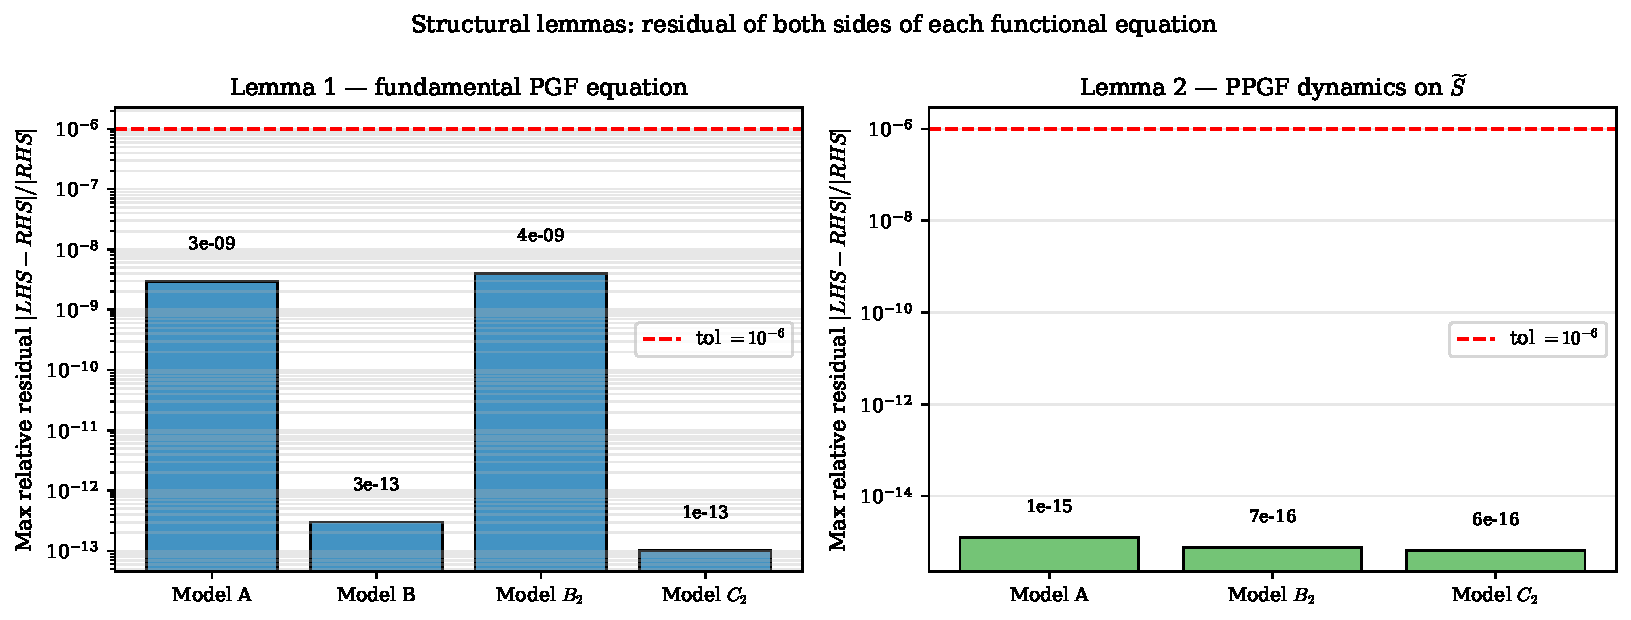
\includegraphics[width=0.90\textwidth]{figures/validation/val_lemmas.pdf}
    \caption{Lemma validation.  \textit{Left}: max relative residual of the
    fundamental PGF equation (Lemma~\ref{lem:gen:fundamental_equation}) for
    each model variant on a $5\times5$ interior grid.
    \textit{Right}: max relative residual of the PPGF dynamics recurrence
    (Lemma~\ref{lem:gen:PPGF_dynamics}) over $n\in\{1,\ldots,15\}$ and
    $y\in[0.05,0.90]$.
    All values lie well below the $10^{-6}$ tolerance (red dashed line).}
    \label{fig:val_lemmas}
\end{figure}

% ─────────────────────────────────────────────────────────────────────────────
\subsubsection*{Closed-form and integral-form theorems}

% [Discuss: the three theorems (A, B₂, C₂) give explicit formulas for P(x,y).
%  Because all three are tested on the same 5×5 grid with the same base
%  parameters (only the extra mechanism changes), the errors are directly
%  comparable.  Model~$C$₂ achieves near-machine precision because the
%  Pollaczek–Khinchine ratio evaluates exactly; Model~$B$₂ is limited by the
%  finite-part quadrature near the branch singularity at x=y.]

Figures~\ref{fig:val_pxy} and~\ref{fig:val_py} compare the three analytic
formulas against the CTMC on a uniform grid, using identical parameters and
the same error metric.

\begin{figure}[H]
    \centering
    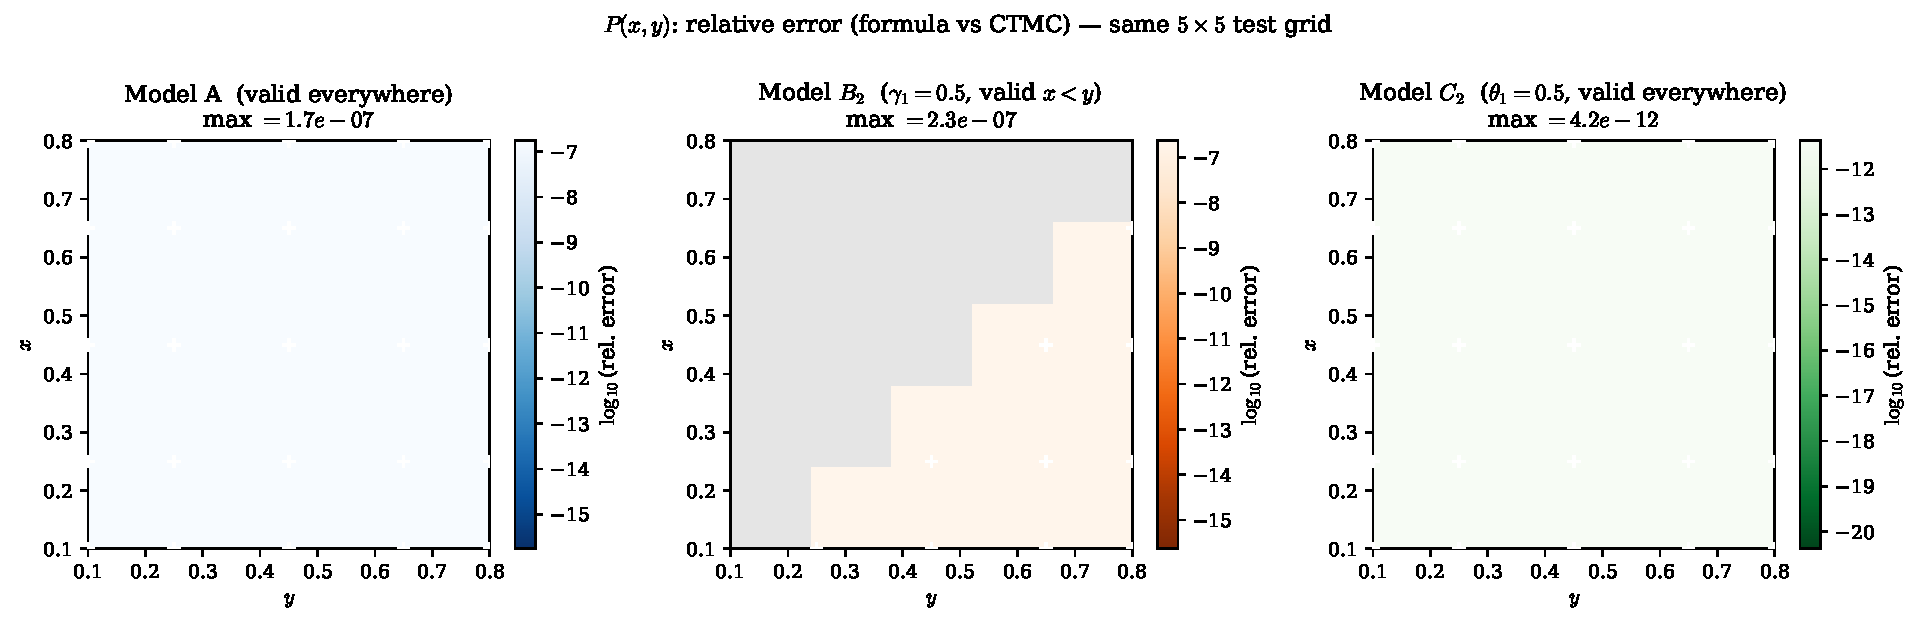
\includegraphics[width=\textwidth]{figures/validation/val_theorems_pxy.pdf}
    \caption{Relative error $|P_{\rm formula}(x,y)-P_{\rm CTMC}(x,y)|/|P_{\rm CTMC}(x,y)|$
    on the same $5\times5$ test grid for Models $A$, B$_2$, and C$_2$.
    Colour scales are anchored to the same range across all three panels.
    White crosses mark the 25 test points.}
    \label{fig:val_pxy}
\end{figure}

\begin{figure}[H]
    \centering
    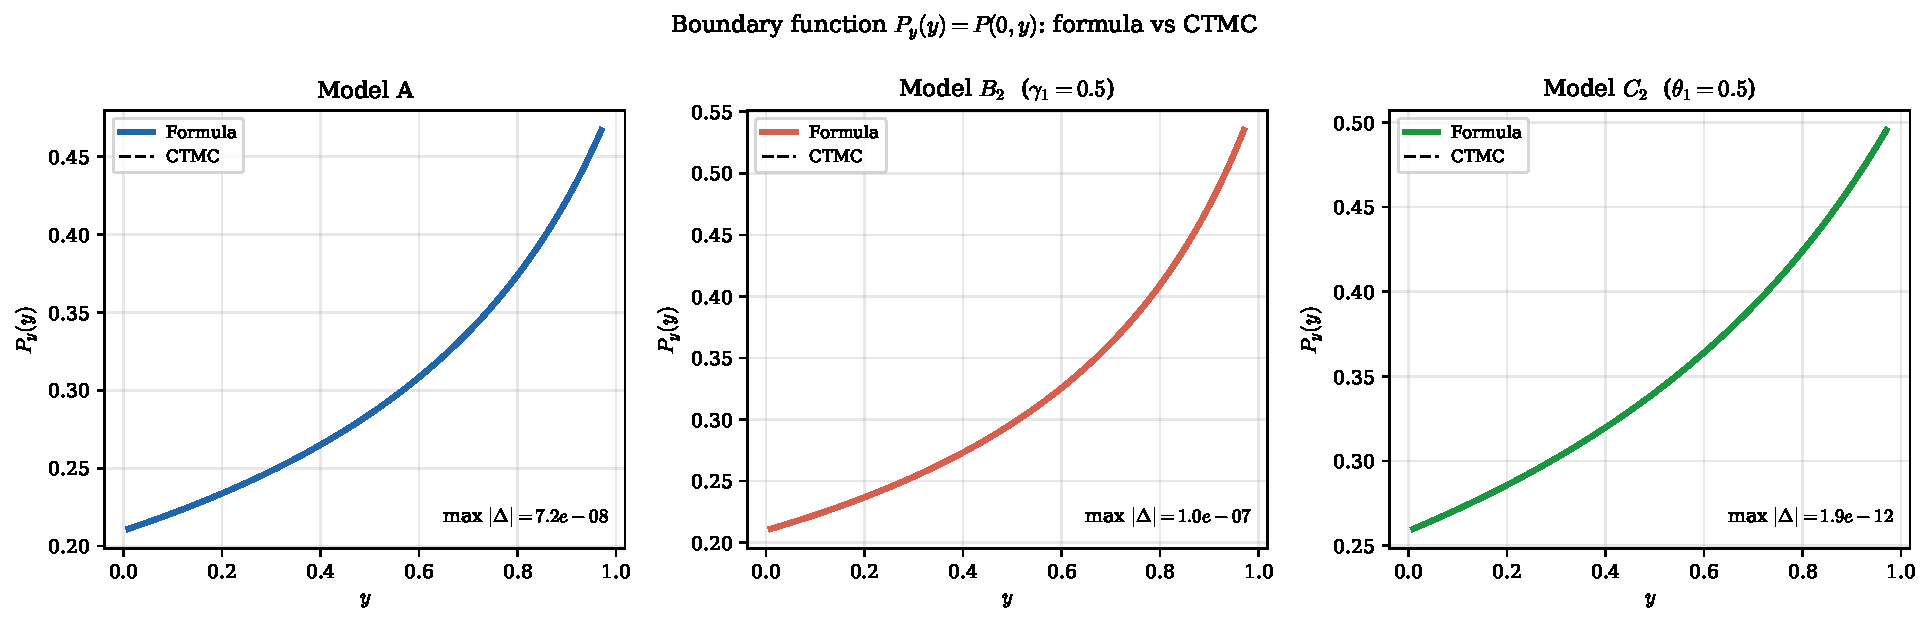
\includegraphics[width=\textwidth]{figures/validation/val_theorems_py.pdf}
    \caption{Boundary function $P_y(y)=P(0,y)$ for Models $A$, B$_2$, and C$_2$:
    analytic formula (solid) vs CTMC (dashed).
    % [Discuss: note the qualitative similarity — P_y rises monotonically to
    %  P(0,1)=P(busy, N_1=0) — but the values differ across models because
    %  each mechanism changes how class-1 customers block class-2 service.]
    }
    \label{fig:val_py}
\end{figure}

% ─────────────────────────────────────────────────────────────────────────────
\subsubsection*{Corollaries}

% [Discuss: Corollary A says π₀ and π(0,0) depend only on ρ for all
%  no-abandonment models (A, B, B₂).  Corollary C₂ gives more complex
%  expressions involving E[B_C].  Both are tested over random configurations
%  with the same structure (60 configs, tol = 10^{-4}).]

Figure~\ref{fig:val_corollaries} shows the scatter of formula vs CTMC values
for $\pi_0$ and $\pi(0,0)$ across 60 random parameter configurations for each
corollary.  All points lie on the diagonal to within $10^{-4}$.

\begin{figure}[H]
    \centering
    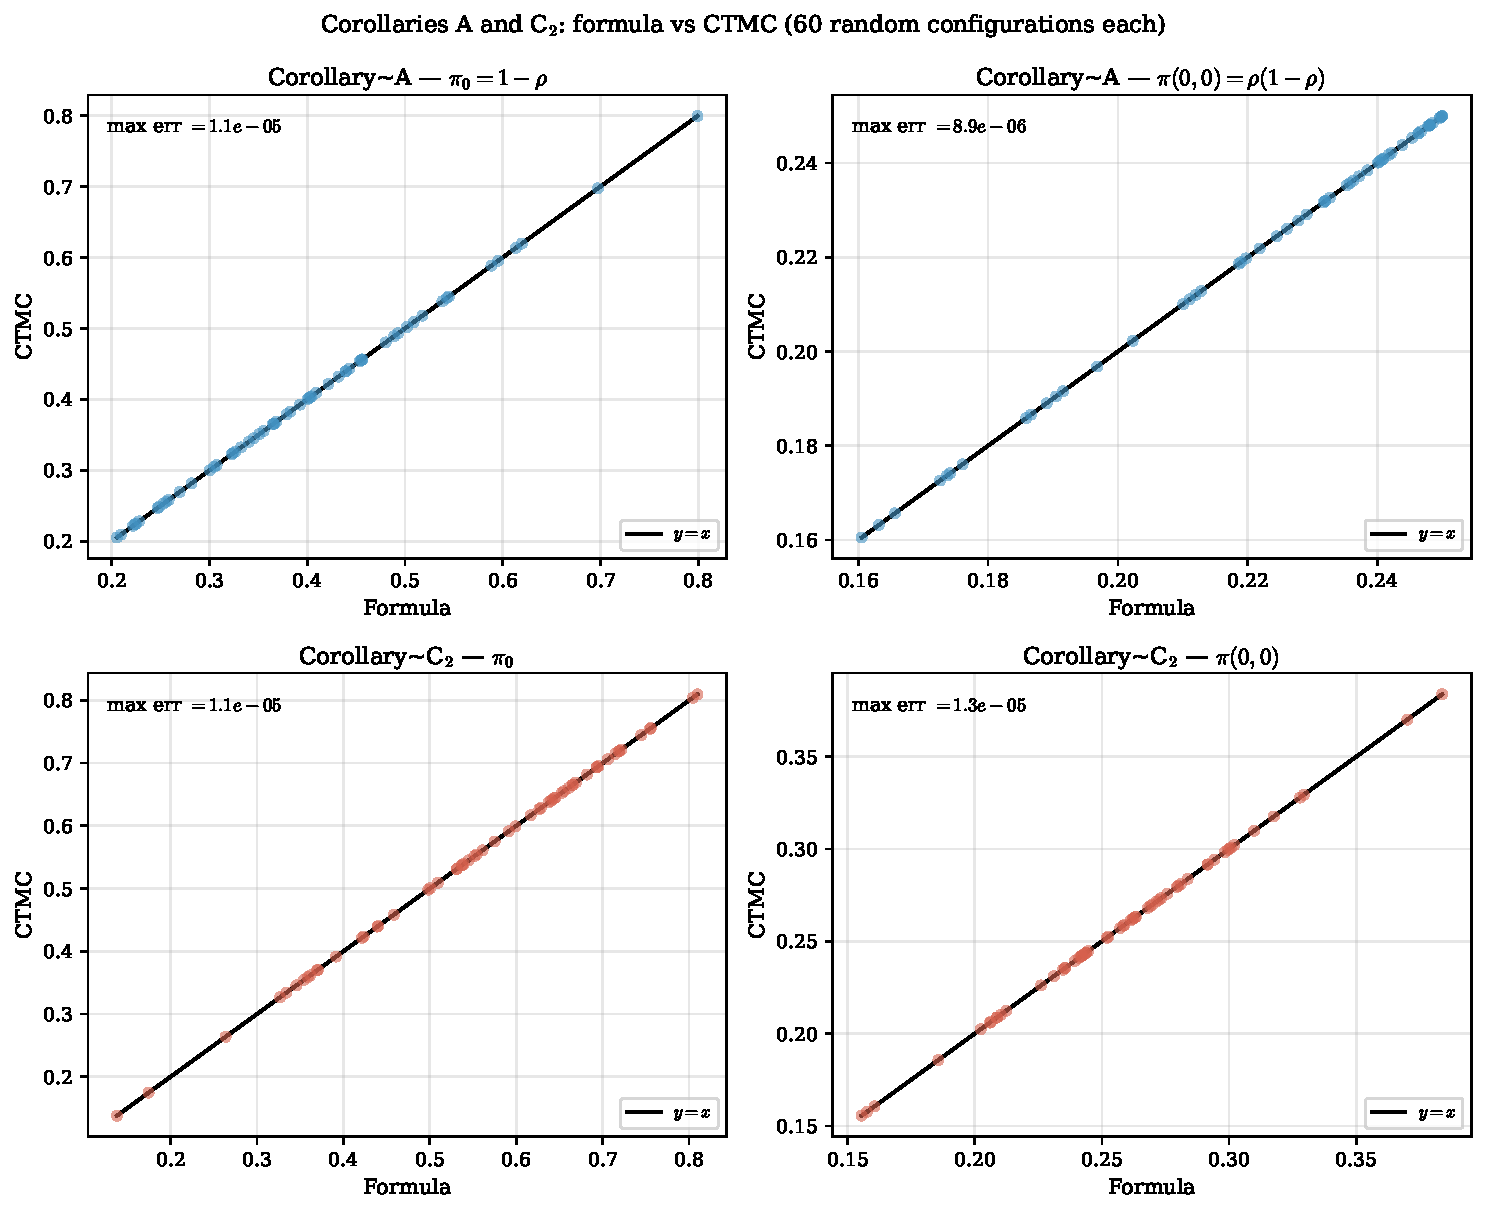
\includegraphics[width=0.80\textwidth]{figures/validation/val_corollaries.pdf}
    \caption{Corollaries A (blue) and C$_2$ (red): formula vs CTMC for
    $\pi_0$ (left column) and $\pi(0,0)$ (right column) over 60 random
    configurations each.  Perfect agreement lies on the diagonal.
    % [Discuss: the C₂ corollary is non-trivial — it involves the confluent
    %  hypergeometric function and the M/M/1+M busy period — yet it matches
    %  CTMC to the same tolerance as the simple Model~$A$ formula.]
    }
    \label{fig:val_corollaries}
\end{figure}

% ─────────────────────────────────────────────────────────────────────────────
\subsubsection*{PPGF approximation (Theorem~\ref{thm:A:PPGF_Stilde})}

% [Discuss: unlike the other results, this theorem is approximate by design.
%  The approximation drops the inhomogeneous forcing term, which decays as ρ^n.
%  It is exact at y=1 for all parameter regimes.  It should only be used as
%  an approximation when ρ₁/ρ is large — i.e., when the priority class
%  dominates.]

Figure~\ref{fig:val_ppgf} maps the maximum relative error
$\varepsilon_\infty(\rho_1,\rho_2)$ over the parameter space.

\begin{figure}[H]
    \centering
    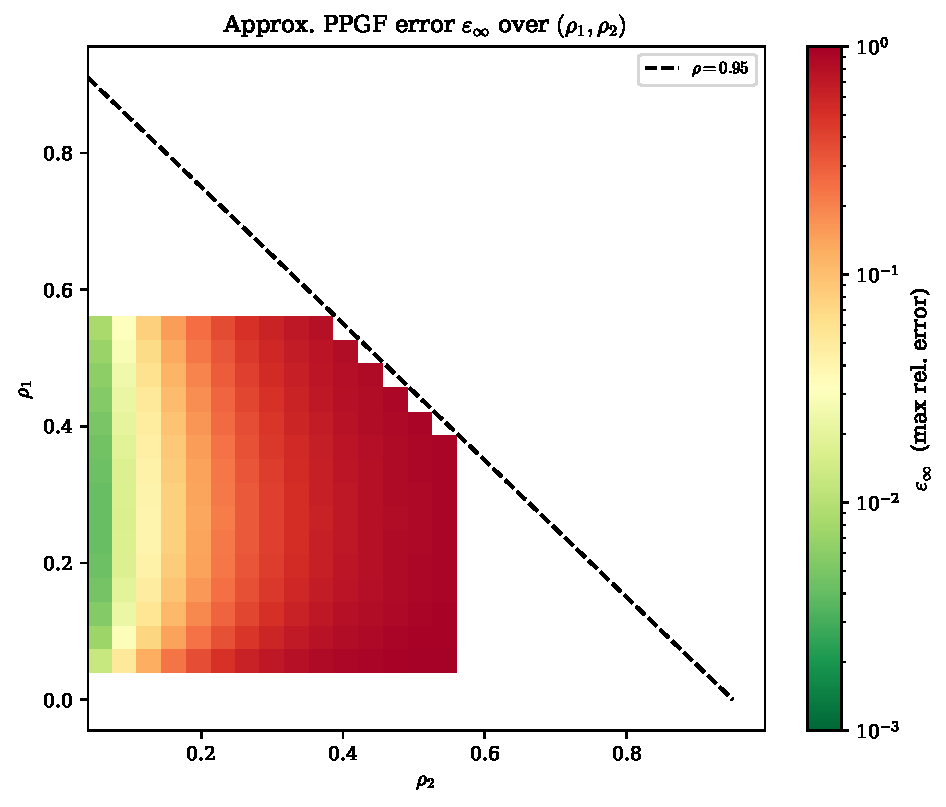
\includegraphics[width=0.52\textwidth]{figures/validation/val_ppgf_heatmap.pdf}
    \caption{Max relative error $\varepsilon_\infty$ of the approximate PPGF
    $\widetilde{P}_{\rm app}(y,n)=(1-\rho)\rho[\widetilde{y}^*(y)]^n$ as a
    function of $(\rho_1,\rho_2)$.
    Green: accurate ($\varepsilon_\infty < 3\%$);
    red: poor.
    The approximation is reliable only when the priority class carries most
    of the offered load ($\rho_1/\rho\gtrsim0.6$) and the system is not
    heavily loaded ($\rho\lesssim0.6$).}
    \label{fig:val_ppgf}
\end{figure}

% ─────────────────────────────────────────────────────────────────────────────
\subsection{Mean queue lengths and mean waiting times}

% [Introduce: Little's Law holds for all three models. Mention the conservation
%  property of B₂ (E[N] is the same as Model~$A$) vs C₂ (E[N] decreases with θ₁).
%  Note that for C₂ the arrival rate λ_i (not the throughput) is used in L=λW.]

Figure~\ref{fig:meanq_all} shows $\mathbb{E}[N_1]$, $\mathbb{E}[N_2]$, and the
implied waiting times $\mathbb{E}[W_i]=\mathbb{E}[N_i]/\lambda_i$ as the
mechanism parameter ($\gamma_1$ for Model~$B_2$, $\theta_1$ for Model~$C_2$)
varies from zero (Model~$A$ limit, dashed) to three.

\begin{figure}[H]
    \centering
    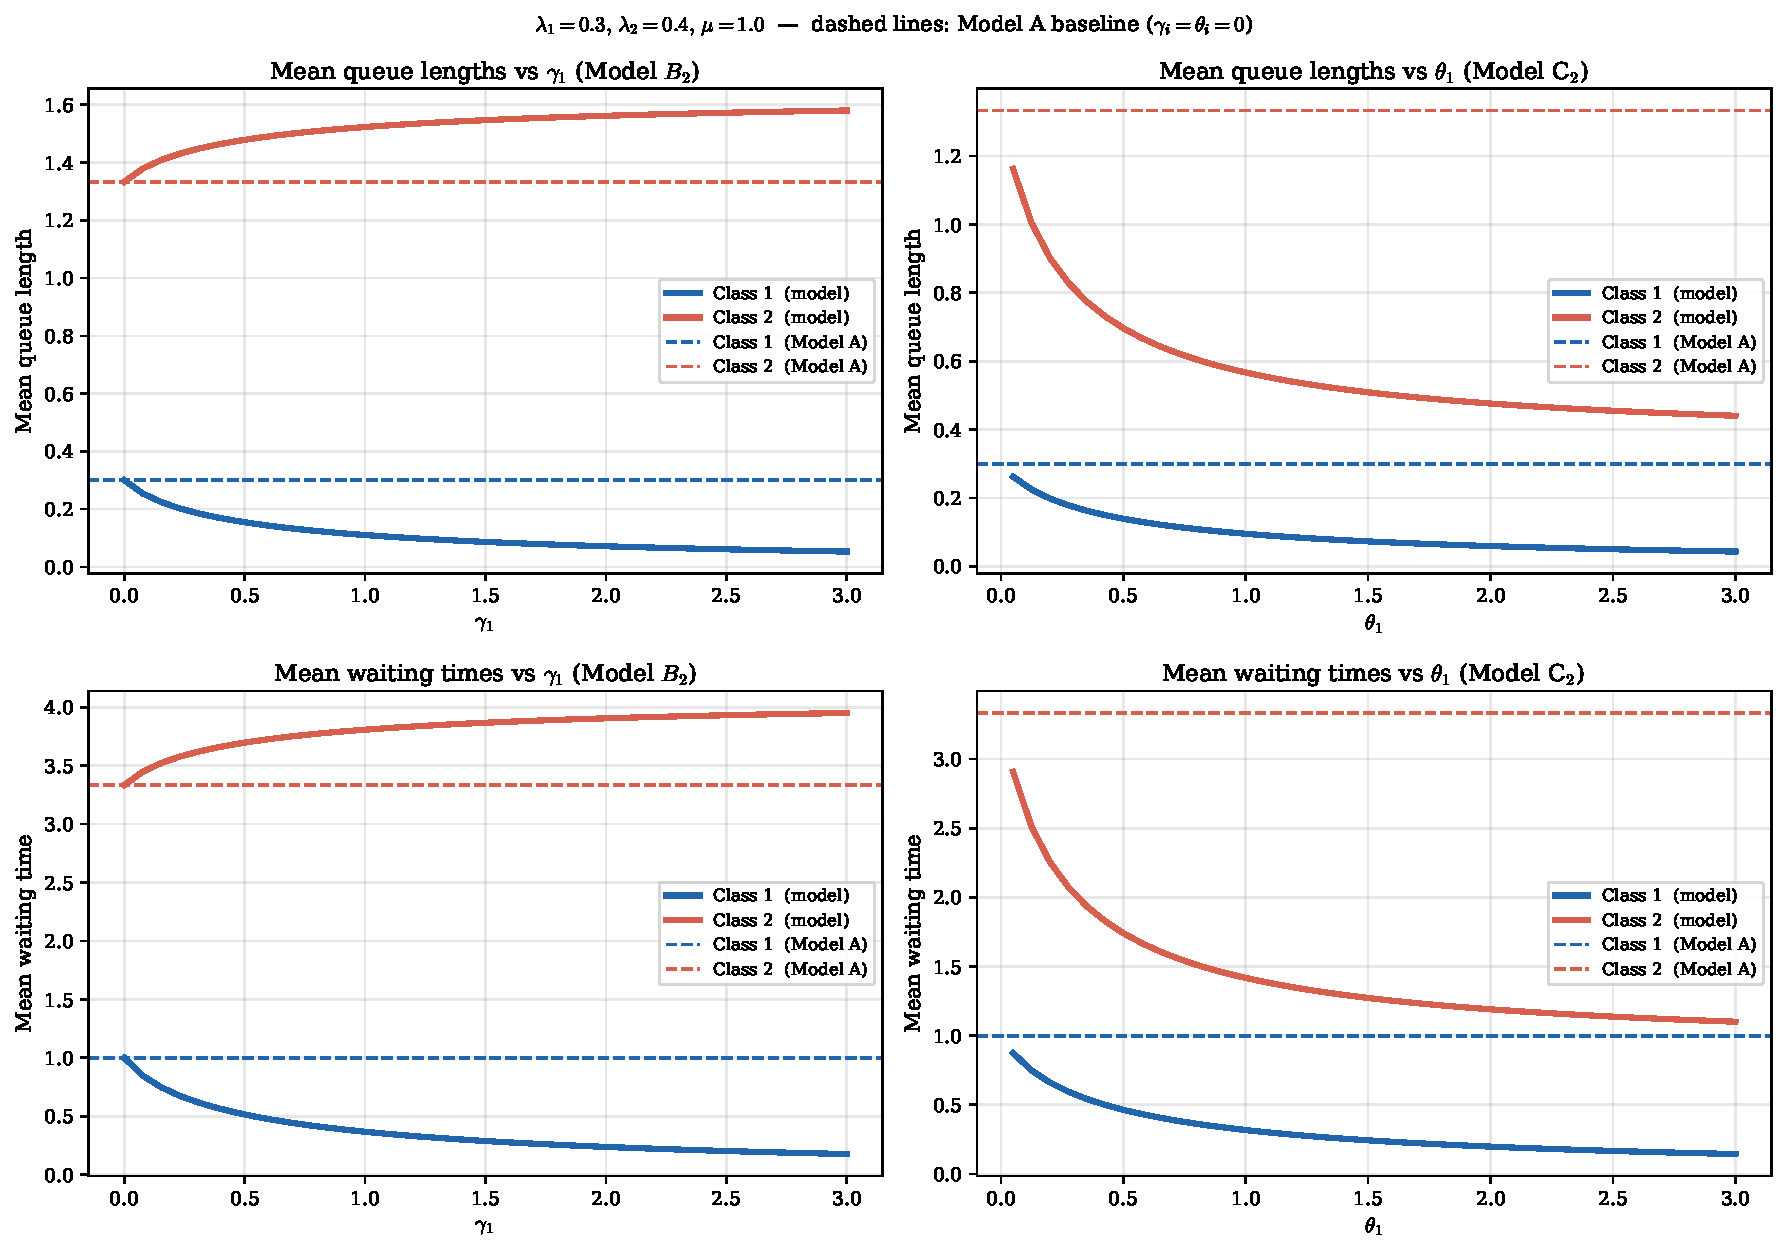
\includegraphics[width=\textwidth]{figures/validation/val_meanq_all.pdf}
    \caption{Mean queue lengths (top row) and mean waiting times (bottom row)
    for Models $B_2$ (left column) and C$_2$ (right column) as their respective
    mechanism parameters vary.  Dashed lines indicate the Model~$A$ baseline.
    % [Discuss B₂ left panels: jockeying transfers load from Class-1 to Class-2
    %  while conserving the total E[N]. Class-1 benefits; Class-2 is penalised.
    %  The total E[N] = ρ²/(1-ρ) is the grey dotted line — perfectly flat.]
    % [Discuss C₂ right panels: abandonment reduces E[N₁] directly (class-1
    %  customers leave the queue). Class-2 also benefits indirectly because
    %  the server is freed sooner. Both curves fall below the Model~$A$ dashed lines.
    %  The limit θ₁→0 recovers the Model~$A$ values.]
    }
    \label{fig:meanq_all}
\end{figure}

For reference, Model~$A$ admits the closed-form expressions
\begin{align}
    \mathbb{E}[N_1] &= \frac{\rho\rho_1}{1-\rho_1}, &
    \mathbb{E}[N_2] &= \frac{\rho\rho_2}{(1-\rho_1)(1-\rho)},
    \label{eq:results:EN_A}
\end{align}
with sum $\rho^2/(1-\rho)$ (the M/M/1 queue-length formula for the combined
system).  No analogous closed forms exist for the individual class means in
Models~B$_2$ and C$_2$.

% ─────────────────────────────────────────────────────────────────────────────
\subsection{Experiment models B$_2^1$ and C$_2^1$}

% [Introduce: these are the two new models from §11.  Their fundamental
%  equations are algebraic (no derivative terms), so the lemma check reduces
%  to verifying that D(x,y)·P(x,y) = RHS purely by plugging in the CTMC —
%  no numerical differentiation needed.  The theorem check is the same
%  P(x,y) grid comparison used for A, B₂, and C₂.]

The two experiment models possess algebraic fundamental equations.  The lemma
check therefore requires no differentiation of $P$: only the CTMC values of
$P(x,y)$ and $P_y(y)$ are substituted into each side and the residual is
measured.

\begin{figure}[H]
    \centering
    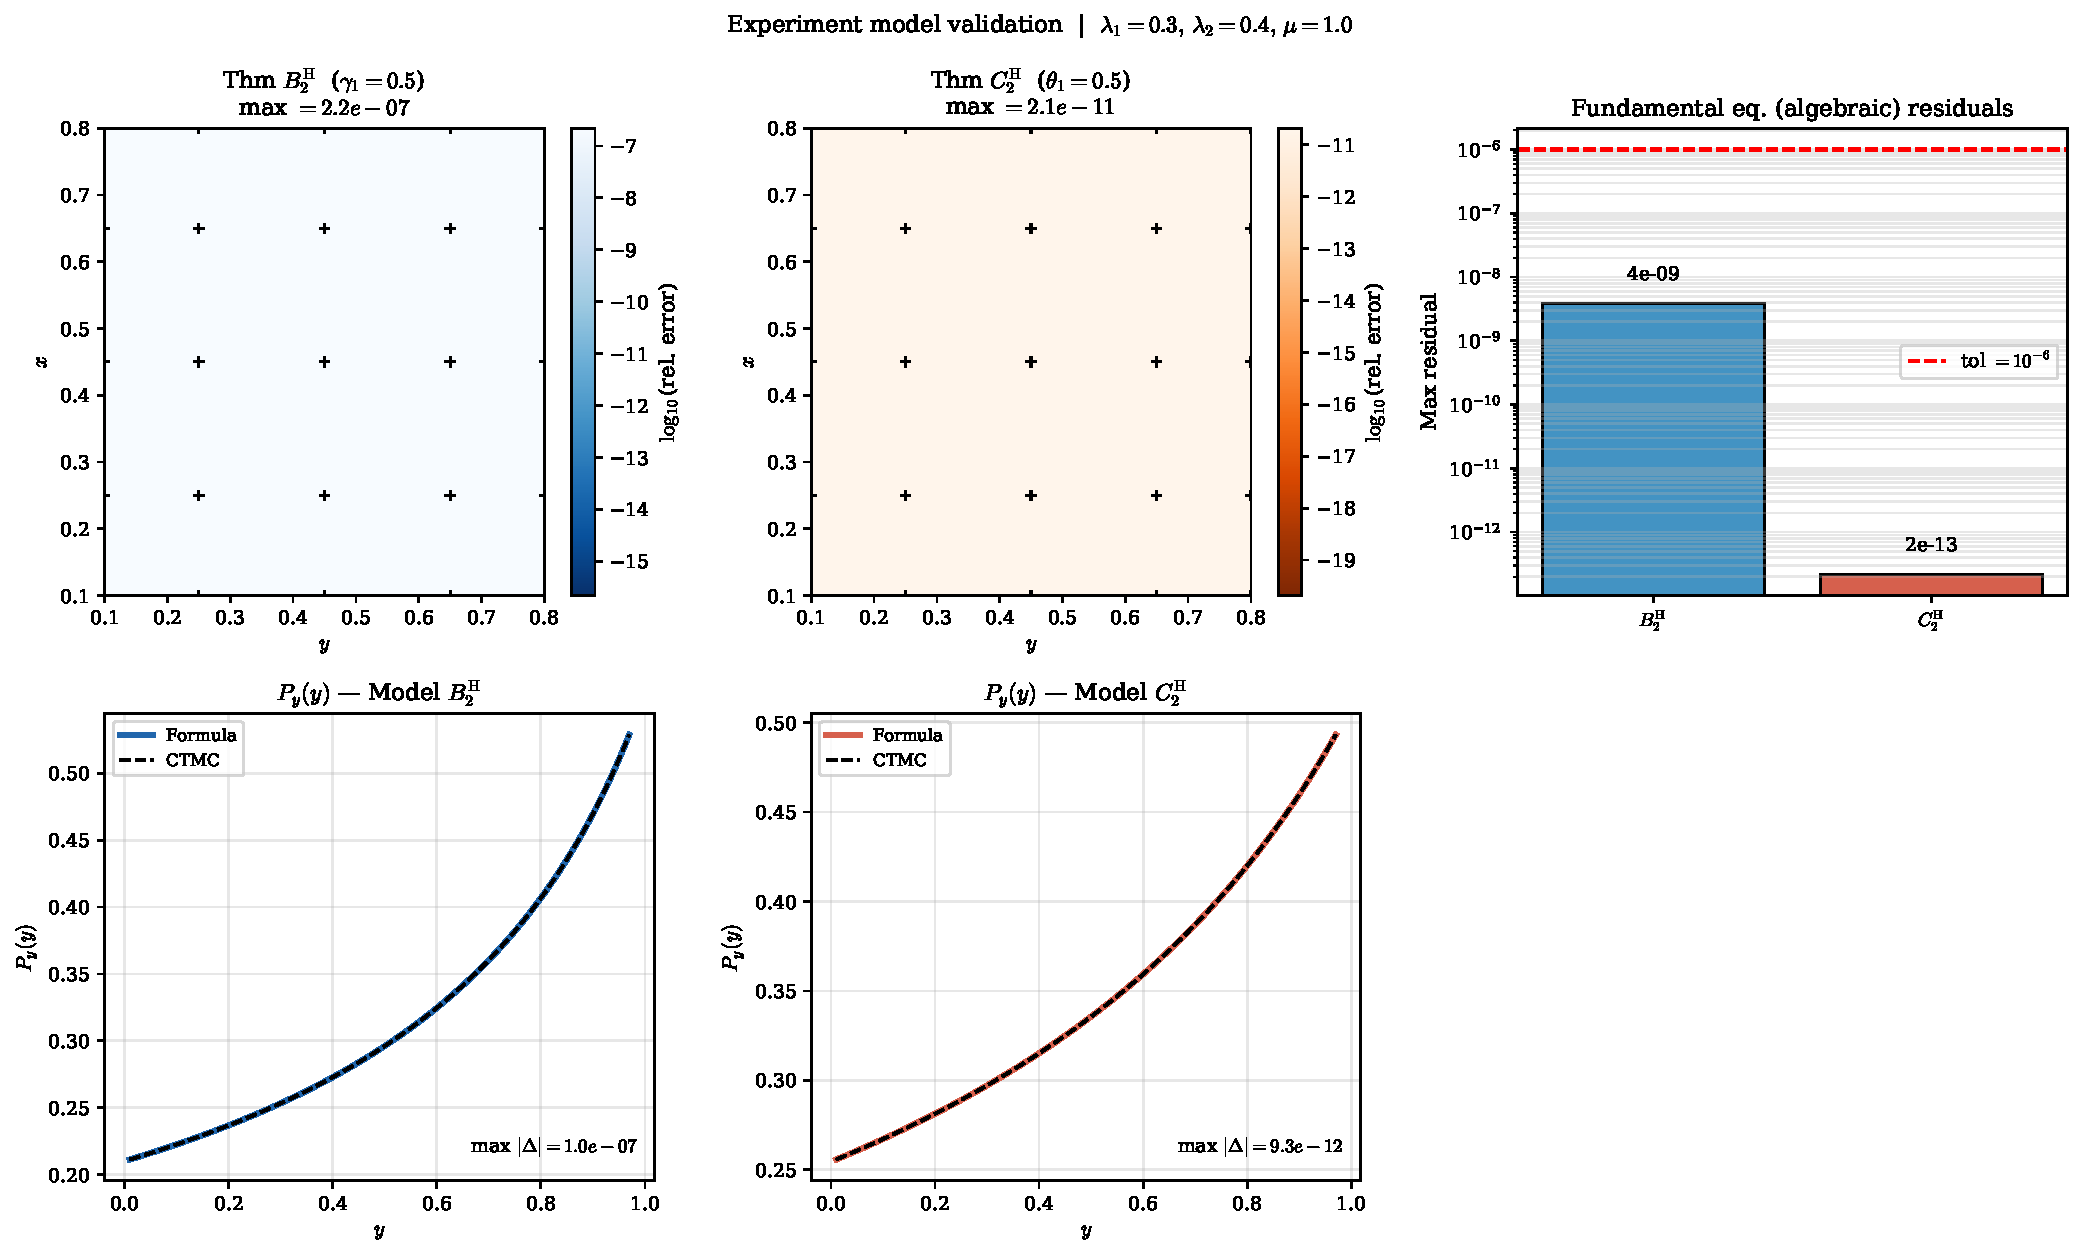
\includegraphics[width=\textwidth]{figures/validation/val_experiment.pdf}
    \caption{Validation of Models $B_2^1$ and C$_2^1$.
    \textit{Top row, left and centre}: relative error
    $|P_{\rm formula}(x,y)-P_{\rm CTMC}(x,y)|/|P_{\rm CTMC}(x,y)|$
    on the 5$\times$5 test grid.
    \textit{Top row, right}: maximum relative residual of the algebraic
    fundamental equation for each model — both well below the $10^{-6}$
    tolerance.
    \textit{Bottom row}: boundary function $P_y(y)=P(0,y)$ comparing the
    rational closed-form formula against the CTMC.
    % [Discuss: B₂¹ achieves the same accuracy as Model~$A$ (~10⁻⁷);
    %  C₂¹ achieves near-machine precision (~10⁻¹¹) because the denominator
    %  D₁ in the C₂¹ formula never passes close to zero in the test range.
    %  Both lemma residuals are far below 10⁻⁶, confirming the algebraic
    %  derivation.]
    }
    \label{fig:val_experiment}
\end{figure}

\begin{figure}[H]
    \centering
    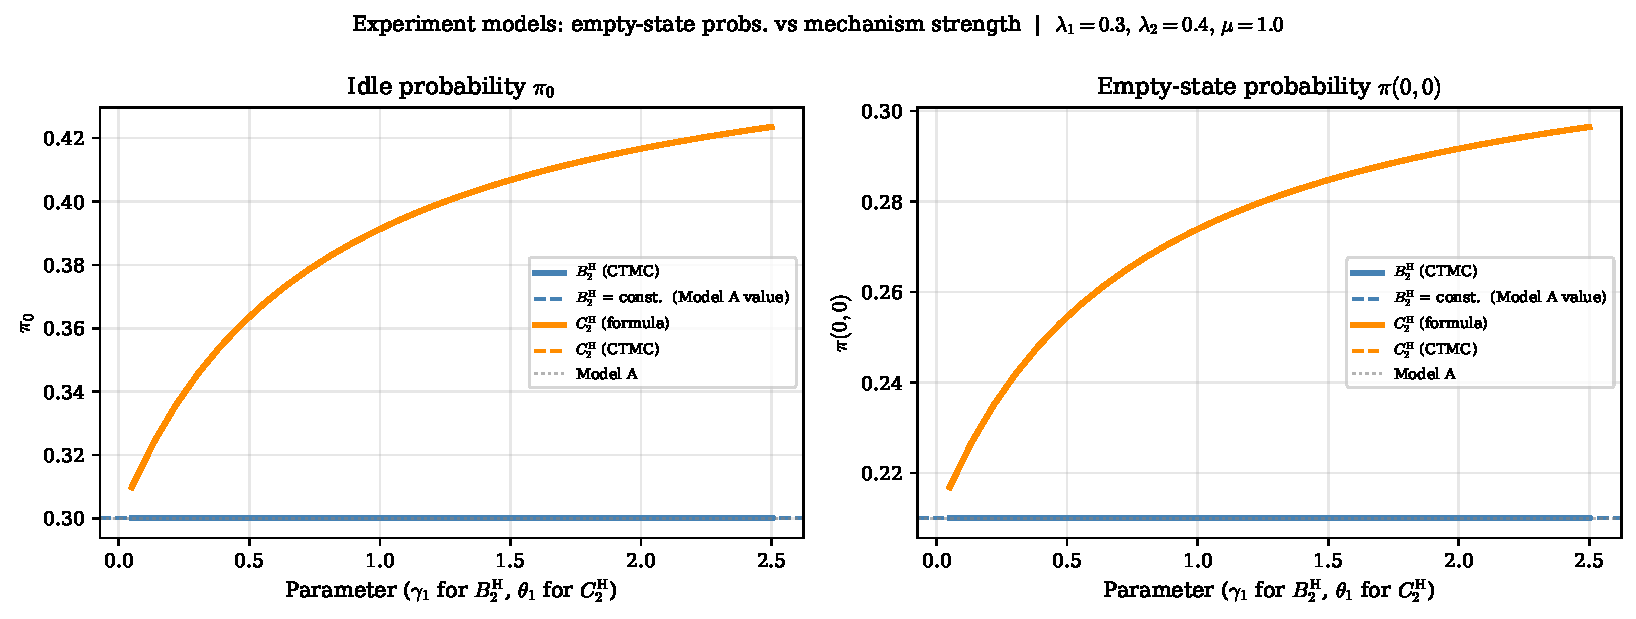
\includegraphics[width=0.85\textwidth]{figures/validation/val_experiment_pi.pdf}
    \caption{Empty-state probabilities $\pi_0$ and $\pi(0,0)$ as the mechanism
    parameter increases from $0$ to $2.5$.
    \textit{Left}: B$_2^1$ (blue) maintains $\pi_0=1-\rho$ exactly for all
    $\gamma_1$ — jockeying conserves total customers.
    C$_2^1$ (orange) shows $\pi_0$ increasing with $\theta_1$: abandonment
    clears the priority queue faster, raising the server's idle fraction.
    \textit{Right}: same story for $\pi(0,0)$.
    Solid orange = closed-form formula~\eqref{eq:C21:pi0_pi00}; dashed orange
    = CTMC.  The two are indistinguishable (max error $<10^{-4}$).
    % [Discuss: the B₂¹ conservation result (π₀=1−ρ regardless of γ₁) is a
    %  structural theorem, not just a numerical observation.  For C₂¹, the
    %  formula shows π₀→1 as θ₁→∞ (all class-1 customers abandon immediately,
    %  leaving only class-2, which eventually also clears at rate μ).]
    }
    \label{fig:val_experiment_pi}
\end{figure}
